\documentclass[12pt,a4paper]{report}
\usepackage{amsmath}
\usepackage[hidelinks]{hyperref}
\usepackage{comment}
\usepackage{graphicx}
\usepackage{placeins}

\usepackage[left=2.50cm, right=2.50cm, top=2.50cm, bottom=2.50cm]{geometry}
\graphicspath{{./Images/}}

\begin{document}
	
	\author{Compliance Design of Automotive Systems \\
		a.y. 2020/2021\\\\
		Group Members:\\
		Barro Alessandro, Bruscoli Nicolas, Ceccarelli Viviana, \\
		Chiacchiararelli Leonardo, Cintura Manuel, Mariani Lucia\\
	}
	\title{Project Report\\
		Adaptive Cruise Control
	}
	\maketitle
	
\tableofcontents
\listoffigures

\chapter{Introduction}

\chapter{Project organization}

\section{Model based design}
\section{Team organization}


\chapter{Model explanation \& design}
As anticipated before, the aim of this project is to design an Adaptive Cruise Control: to design it following the MBD, we of course need a plant that models the vehicle longitudinal dynamics.
In Fig \ref{Plant} it is possible to see the whole plant model.

\begin{figure}[htbp]
	\centering
	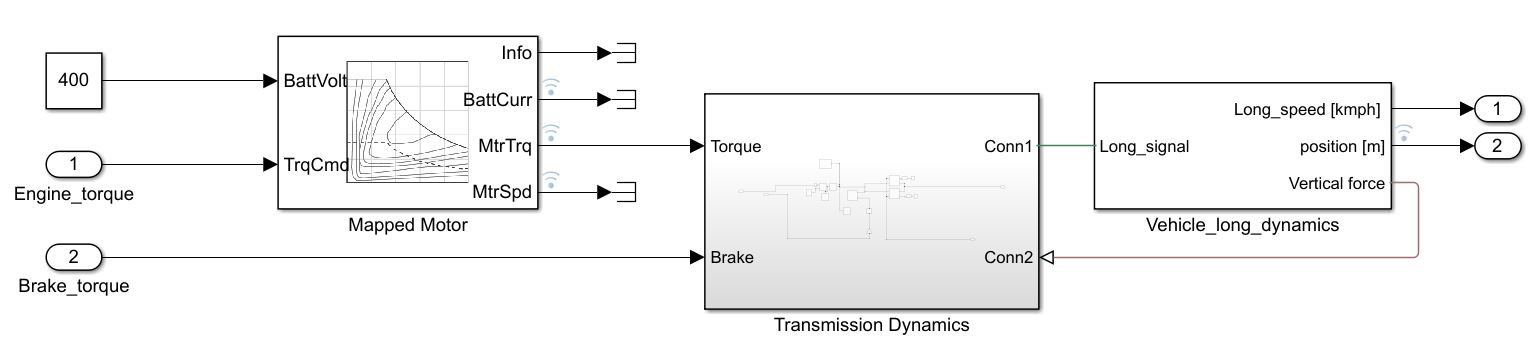
\includegraphics[scale=0.5]{Plant.jpg}
	\caption{Plant}
	\label{Plant}
\end{figure}


Going deeper, to model the longitudinal dynamics of the vehicle we picked from the Simscape Driveline library the “vehicle longitudinal dynamics” block.


We wanted to make some more detailed simulation so we decided to model the driveline system.

The vehicle dynamics block accepts as input the long speed of the vehicle, we associated it to the long speed of the CoG of the wheels.

The simscape wheels block model the behaviour of a the wheel in terms of inertia, rolling resistance and slip. The angular speed of the wheel is proportional to the torque given as input.

The torque is the output of a mapped motor block, of course modified by a gear ratio block that models the one-speed transmission of the electric vehicle.

When a negative torque is asked, the brake block provides a negative torque at the wheel input.

With this plant model we wanted to model the entire driveline from the ECU torque request to the wheels motion.

\chapter{Project development}

\section{Requirements}
\subsection{Software requirements}

In order to be able to interact with the developed model, some software tools are needed:

\begin{itemize}
	
	\item Matlab R2019b;
	
	\item Simulink;
	
	\item Simscape;
	
	\item Simscape Driveline.
	
\end{itemize}

\subsection{High level requirements}

The goal of the overall control system is to extend the mission of the simpler Cruise Control: regulate the speed to the desired one and keep it. In addition respect this goal, the Adaptive Cruise Control adapts the speed of the vehicle respect the velocity of the following one, being able to correctly mantain the safety distance dictated by the Highway Code when it needed (that is to say, when the current distance between the vehicles is lower than the required safety distance):

\begin{equation*}
	d_s=d_{min}+\dfrac{1}{k}v^2
\end{equation*}

\begin{figure}[htbp]
	\centering
	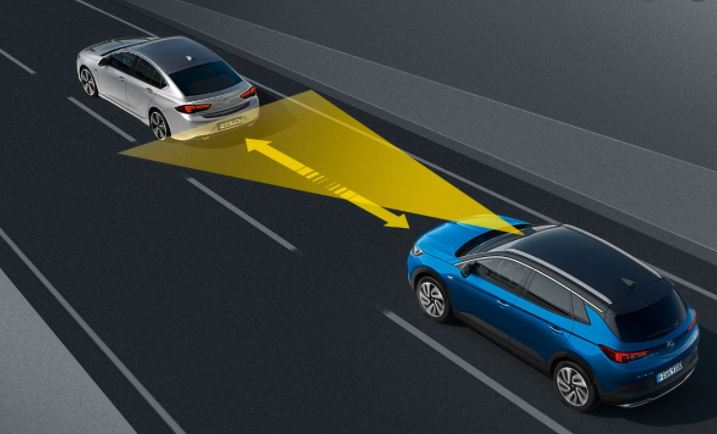
\includegraphics{ACC.jpg}
	\caption{ACC}
\end{figure}

\subsection{Low level requirements}
The designed system is intended to work on an electric vehicle, considering also the state of charge of the battery: particularly, the overall behaviour of the control action will be more or less aggressive depending on the state of charge level.

\begin{figure}[htbp]
	\centering
	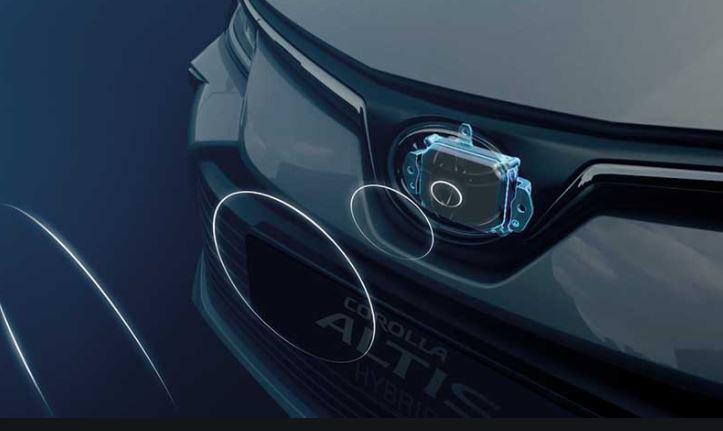
\includegraphics{RadarACC.jpg}
	\caption{Front radar}
\end{figure}

Thanks to the presence of a sensor (typically a radar installed in the front of the car), the distance respect the following vehicle is continuosly monitored: when this distance falls below the threshold dictated by the Highway Code minus a safety margin quantity (one meter as dictated by requirement, to be sure to be able to brake in the correct timings), the control must act on the brakes. Then, during the acceleration phase, the system needs to be designed as following: when the first vehicle accelerates, the control must operate so that the vehicle speed becomes the one desired if it is possible,  that is to say if the two vehicles are far enough. Otherwise, the system must adequate the vehicle speed to the one needed to keep the safety distance.




\section{Unity \& Integration testing}
\begin{figure}[!h]
	\centering
	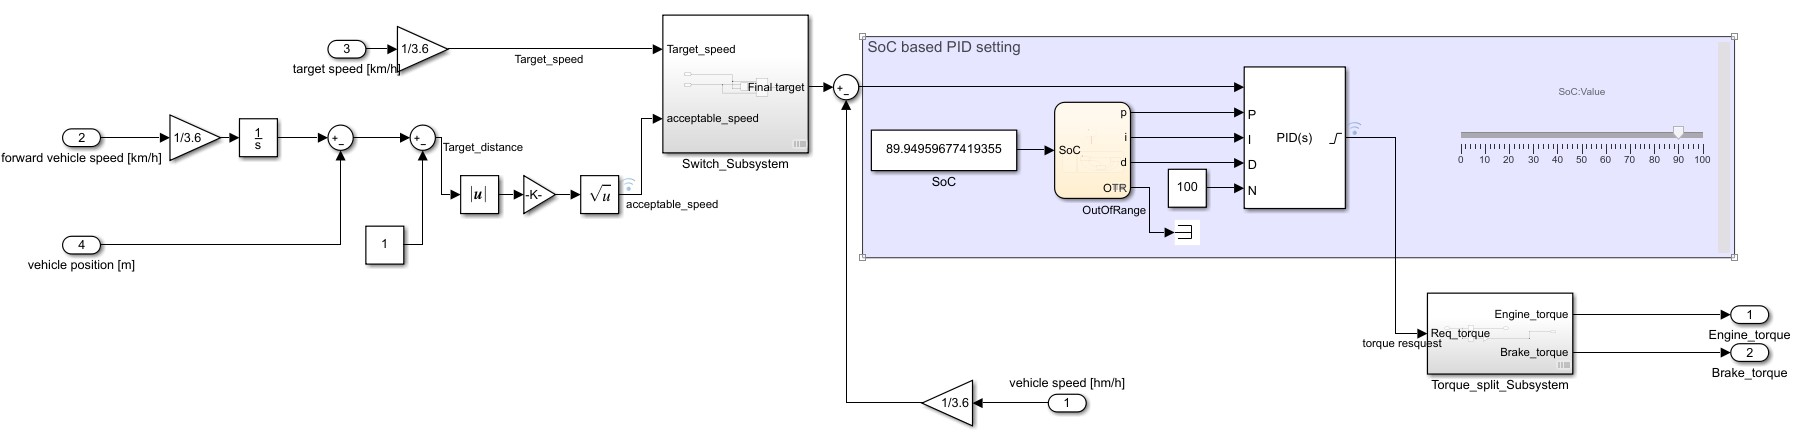
\includegraphics[scale=0.34]{Controller_overview.jpg}
	\caption{An overview of the controller block}
	\label{Controller_overview}
\end{figure}
Our controller is composed by 4 main blocks: switch\_subsys, SoC handler, torque\_split and the PID regulator.
While it is impossible to test the PID behaviour without a model to be controlled, it is necessary to test separately the other blocks.
We tested the units using the tool Simulink Test. We first built an harness for each unity to isolate it from the rest of the model, then we built the input signals in such a way to stimulate the unity in all possible conditions. We also built the baseline signals to tell the tester what output we expected when feeding the unity with a given input. 
\newpage
\subsection{Switch subsystem}
\begin{figure}[!h]
	\centering
	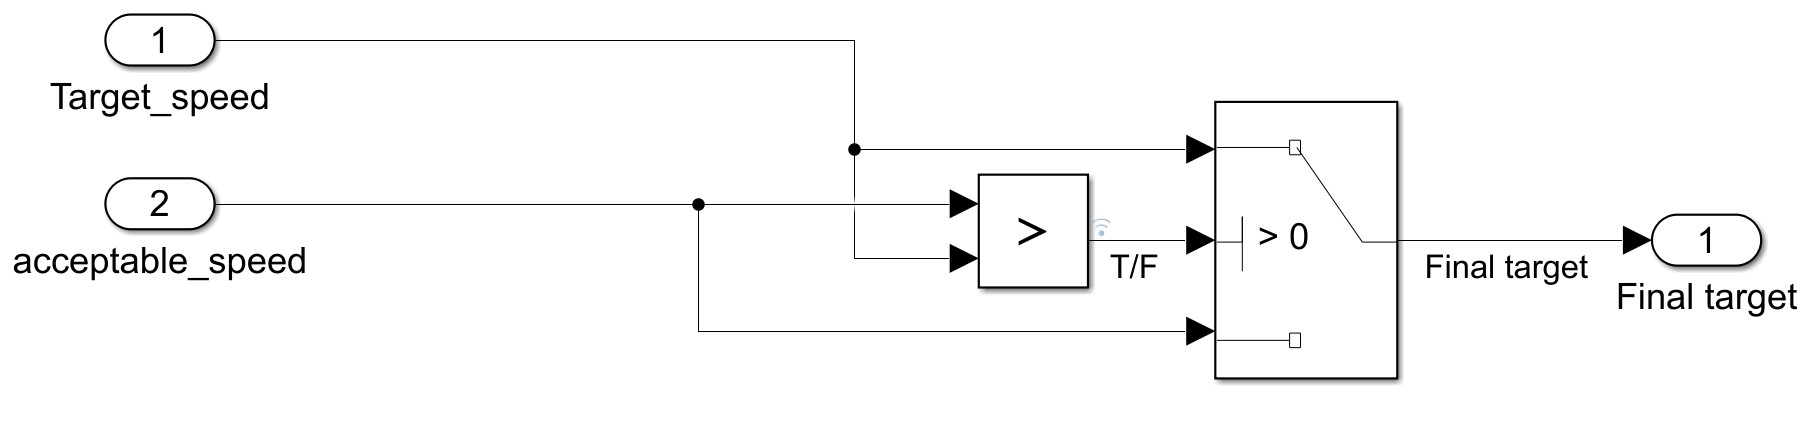
\includegraphics[scale=0.34]{switch_subs.jpg}
	\caption{An overview of the switch subsystem}
	\label{switch_subs}
\end{figure}
\FloatBarrier
This system is composed of a switch commanded by a majority operetor fed with the same signals that have to be switched. We wanted to be shure that this small unity would have behaved as expected. 
In Fig \ref{IO_baseline_switch_detach} we can see the inputs that we used to test the unit: we wanted to test all the possible conditions for the ‘grater than’ block. To better visualize wich signal was let pass by the sitch we ttried to differenciate as much as possible the two inputs.
\begin{figure}[!h]
	\centering
	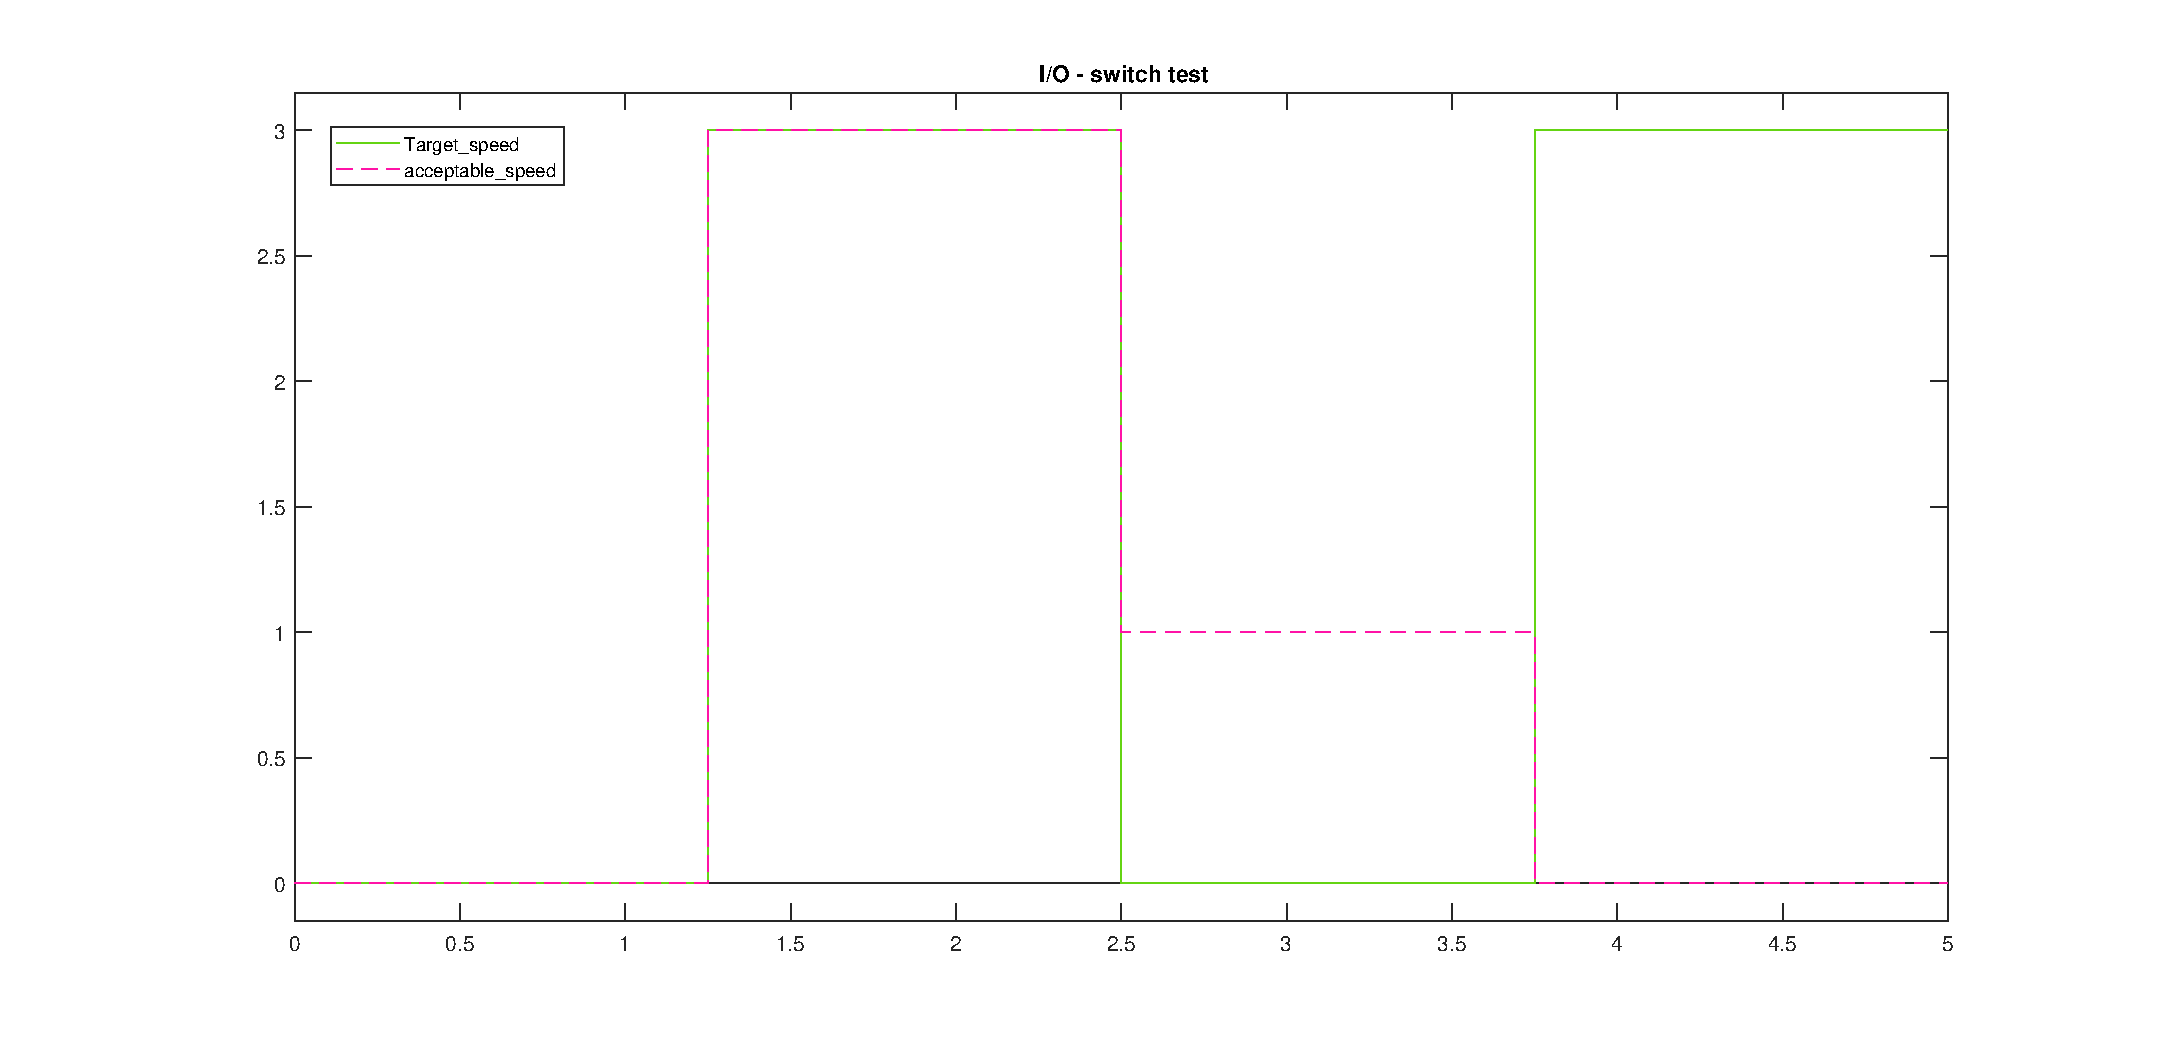
\includegraphics[scale=0.4]{IO_baseline_switch_detach.eps}
	\caption{Inputs of the test: acceptable speed is the one set by the user, target speed is the one of the care ahead}
	\label{IO_baseline_switch_detach}
\end{figure}
As we can see [FIGURE] the simulink test tool is able to generate a document reporting the configuration of the test, to guarantee to the customer (we can call costumer whoever will need to use our subsystem and will need it being tested) that the test was performed accordingly to his needs. This feature also gives the opportunity to an external part to perform the exact same test and verify that the results are coherent.
In the same way the tool can generate a report regarding the output of the test, here in Fig. \ref{switch_baseline} we can see that the test produces successful results, infact the output of the test coincides precisely with our baseline signal. 
%PUT BOTH THE FIGURES IN ONE FIGURE SIDE BY SIDE
\begin{figure}[!h]
	\centering
	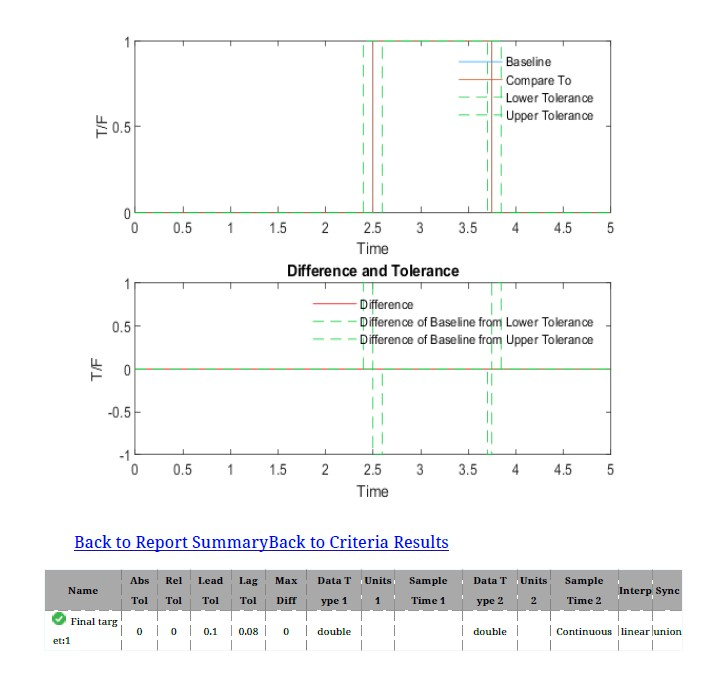
\includegraphics[scale=0.4]{switch_baseline.jpg}
	\caption{Automatiacally generated test reports}
	\label{switch_baseline}
\end{figure}
\FloatBarrier
\subsection{Torque split}
\begin{figure}[!h]
	\centering
	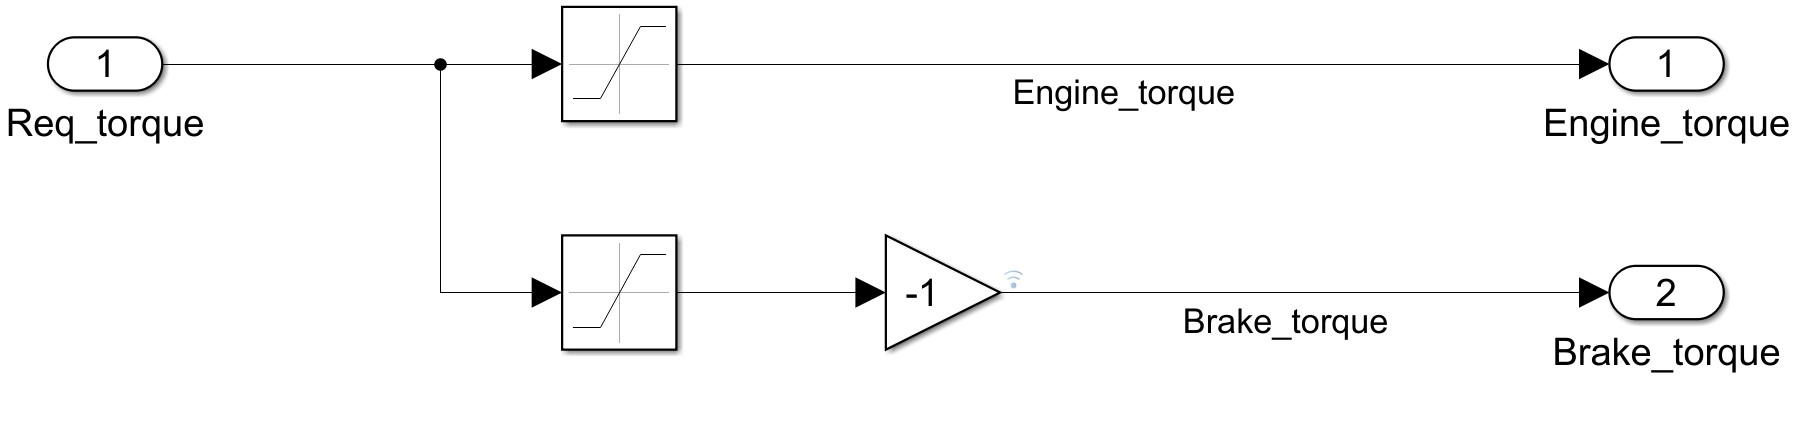
\includegraphics[scale=0.34]{split_subs.jpg}
	\caption{An overview of the torque split subsystem}
	\label{split_subs}
\end{figure}
This unit’s goal is to split the signal coming from the PID, asking for torque. The PID asks for a negative or positive torque, we have to be able to translate the negative torque in a signal to be sent to the brake module. This unit’s goal is to devide the torque signal into two signals depending on the sign of the PID output. To test this unit we just had to verify that when given a positive input it was tranferred to output assigned to the engine and when given a negative input it was transferred to the brake output. At the same time the ouput assigned to the opposite sign has to be zero.
In Fig. \ref{input_split_test} you can see how the test input was designed and you can see that the output corresponds exacly to the baseline signal, meaning a successful test.
\begin{figure}[!hbt]
	\centering
	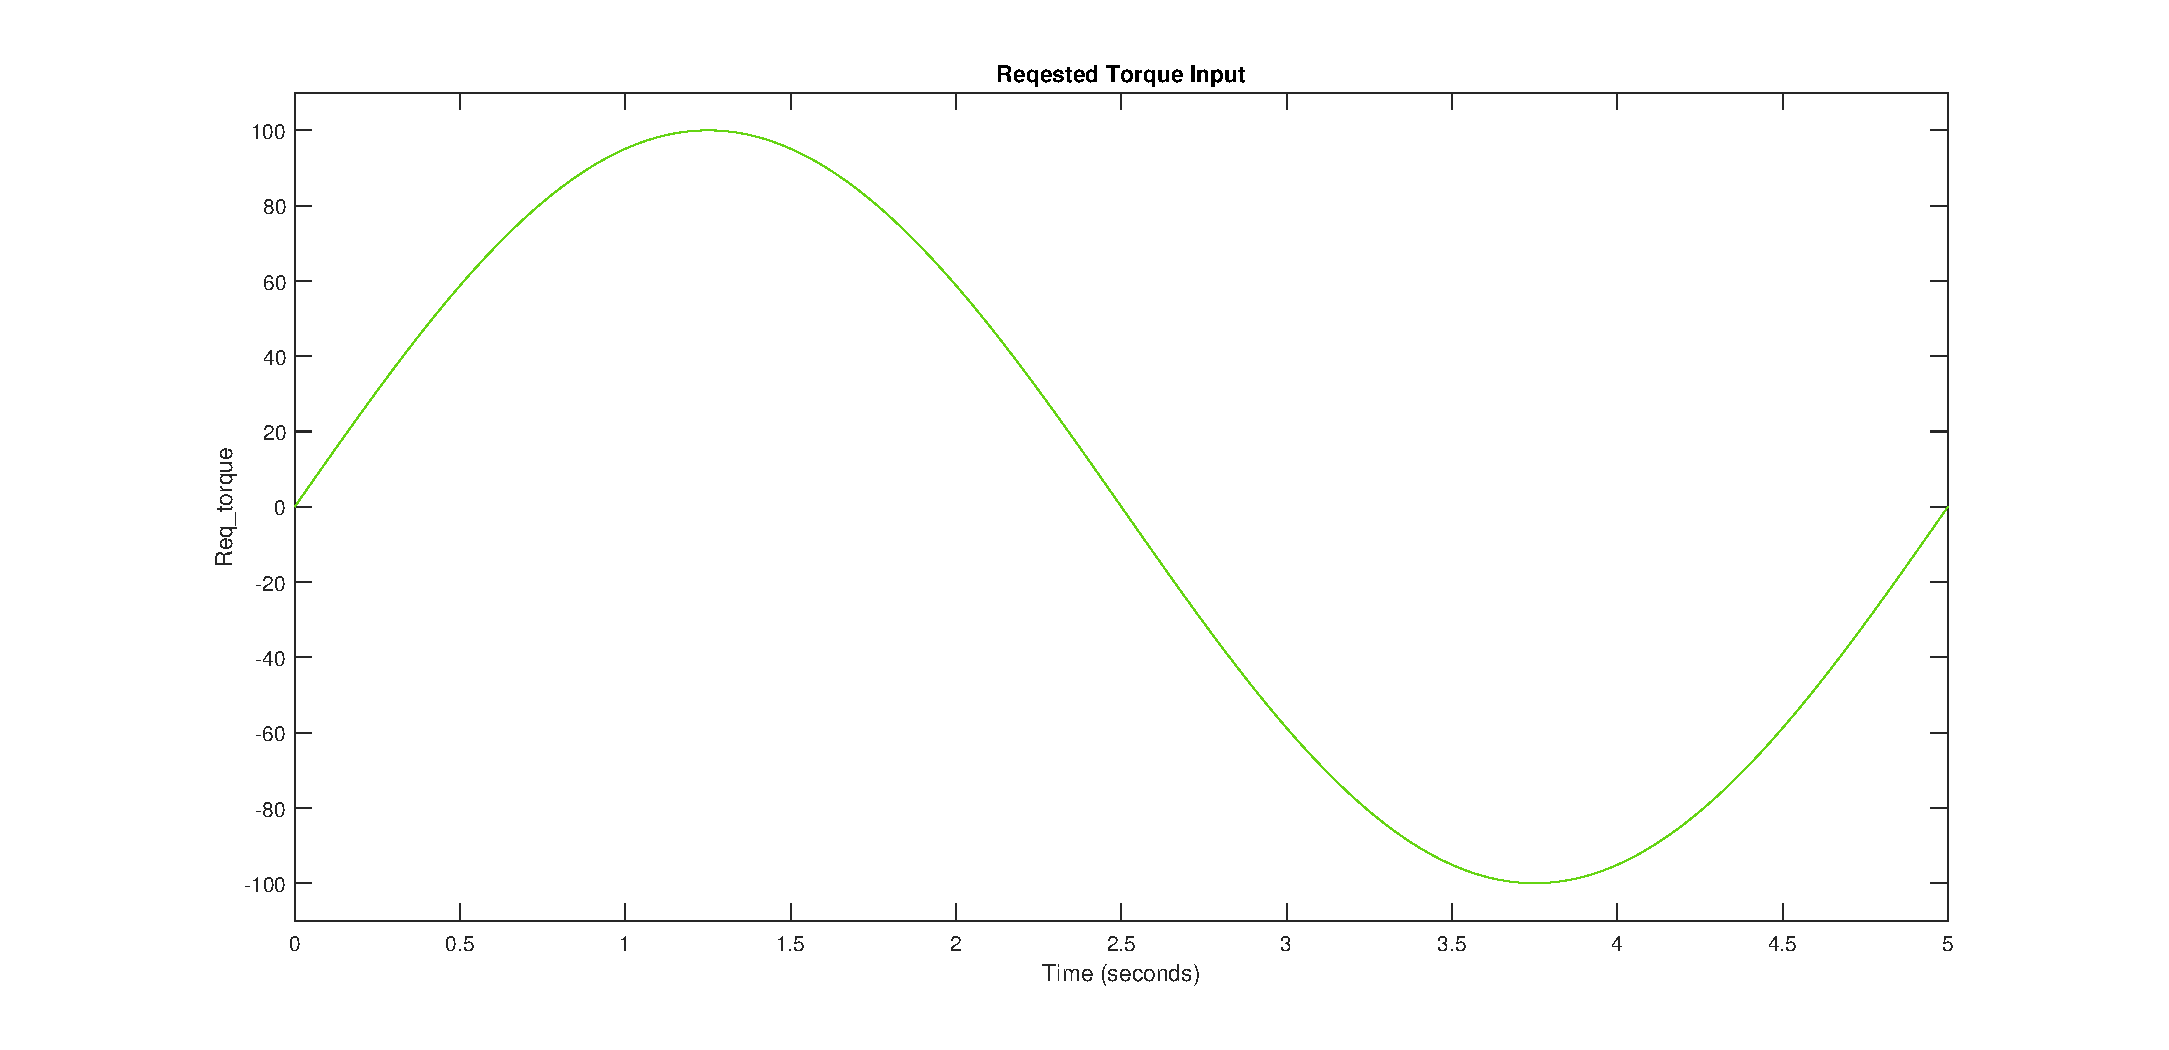
\includegraphics[scale=0.4]{input_split_test}\hfill
	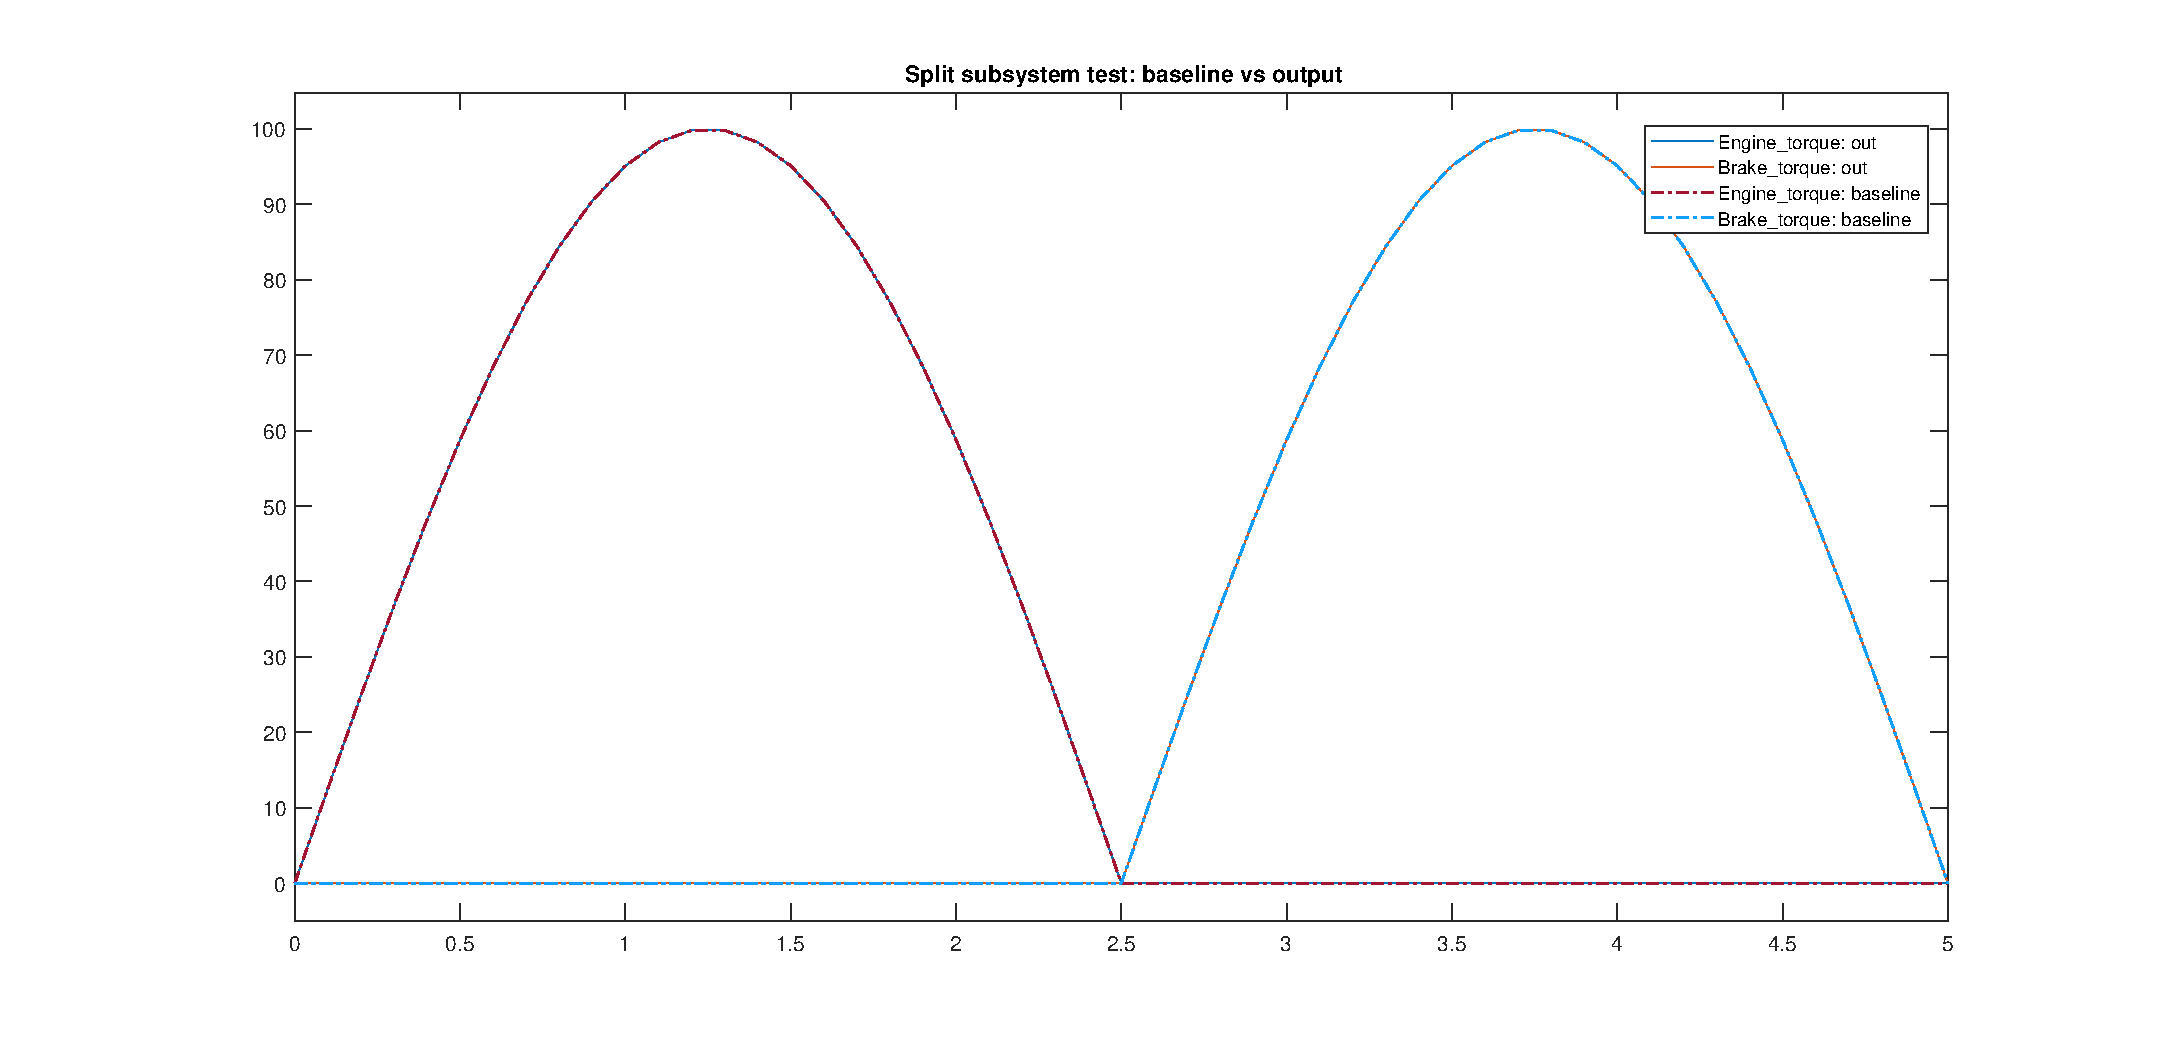
\includegraphics[scale=0.4]{out_split_test}
	\caption{Test inputs (up) Outputs vs baseline (down)}
	\label{input_split_test}
\end{figure}
\FloatBarrier
\subsection{SoC handler}
\begin{figure}[!h]
	\centering
	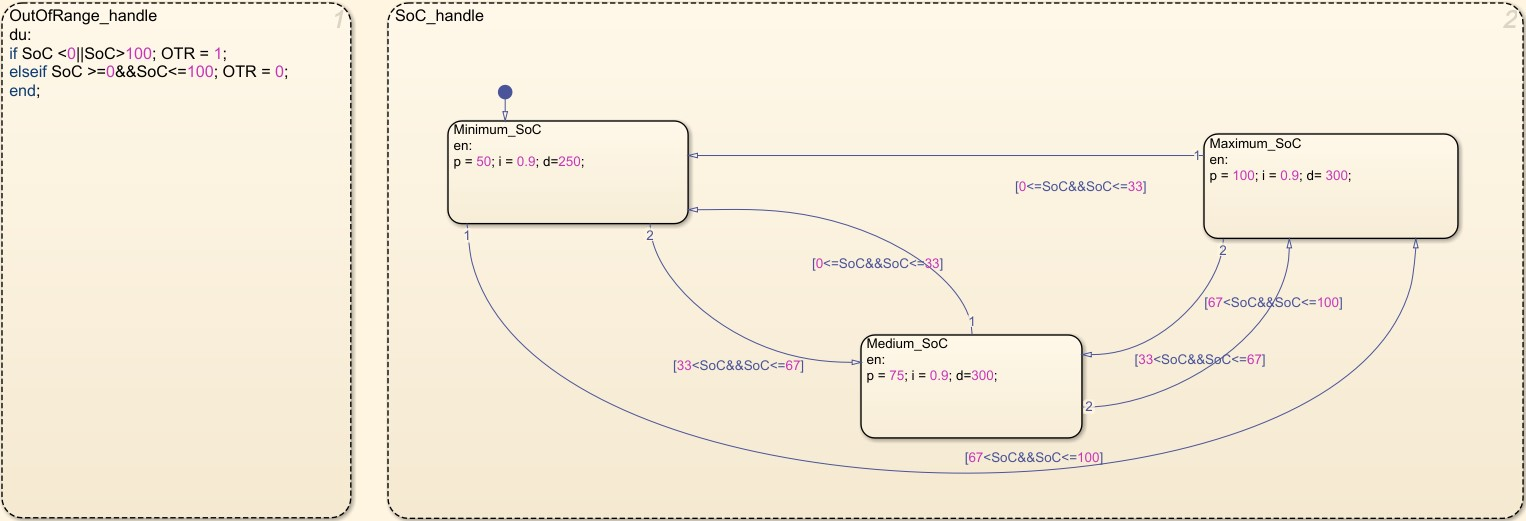
\includegraphics[scale=0.34]{SoC_handle_subs.jpg}
	\caption{An overview of the SoC handler chart}
	\label{SoC_handle_subs}
\end{figure}
\FloatBarrier
This unit is a FSM, so a slightly more complicated test is due. The goal of this uniti s to manage the aggressiveness of the control depending on the SoC of the vehicle’s battery pack. We want a less aggressive control if the car has less autonomy left. We divided the interval of possible SoC values in three segments: minumum, medium, maximum. Each segment corresponds to a different state. We have three states, since from each state you can go to the other two we have in total 6 transitions.  We have only one input: SoC signal. In the input signal, wich you can see in Fig.\ref{SoC_handle_input}, we changed the signal in order to stimulate all the possible transitions. 
To be more robust against unexpected behaviour we wanted an additional output for the FSM. The SoC signal is expected to never trespass the 0\% and 100\% bounds, so we created a signal “OutOfRange” that rises when this condition is verified. The FSM is designed to check constantly the OTR signal while performing the ordinary tasks, so a parallel state is created in the FSM.
\begin{figure}[!h]
	\centering
	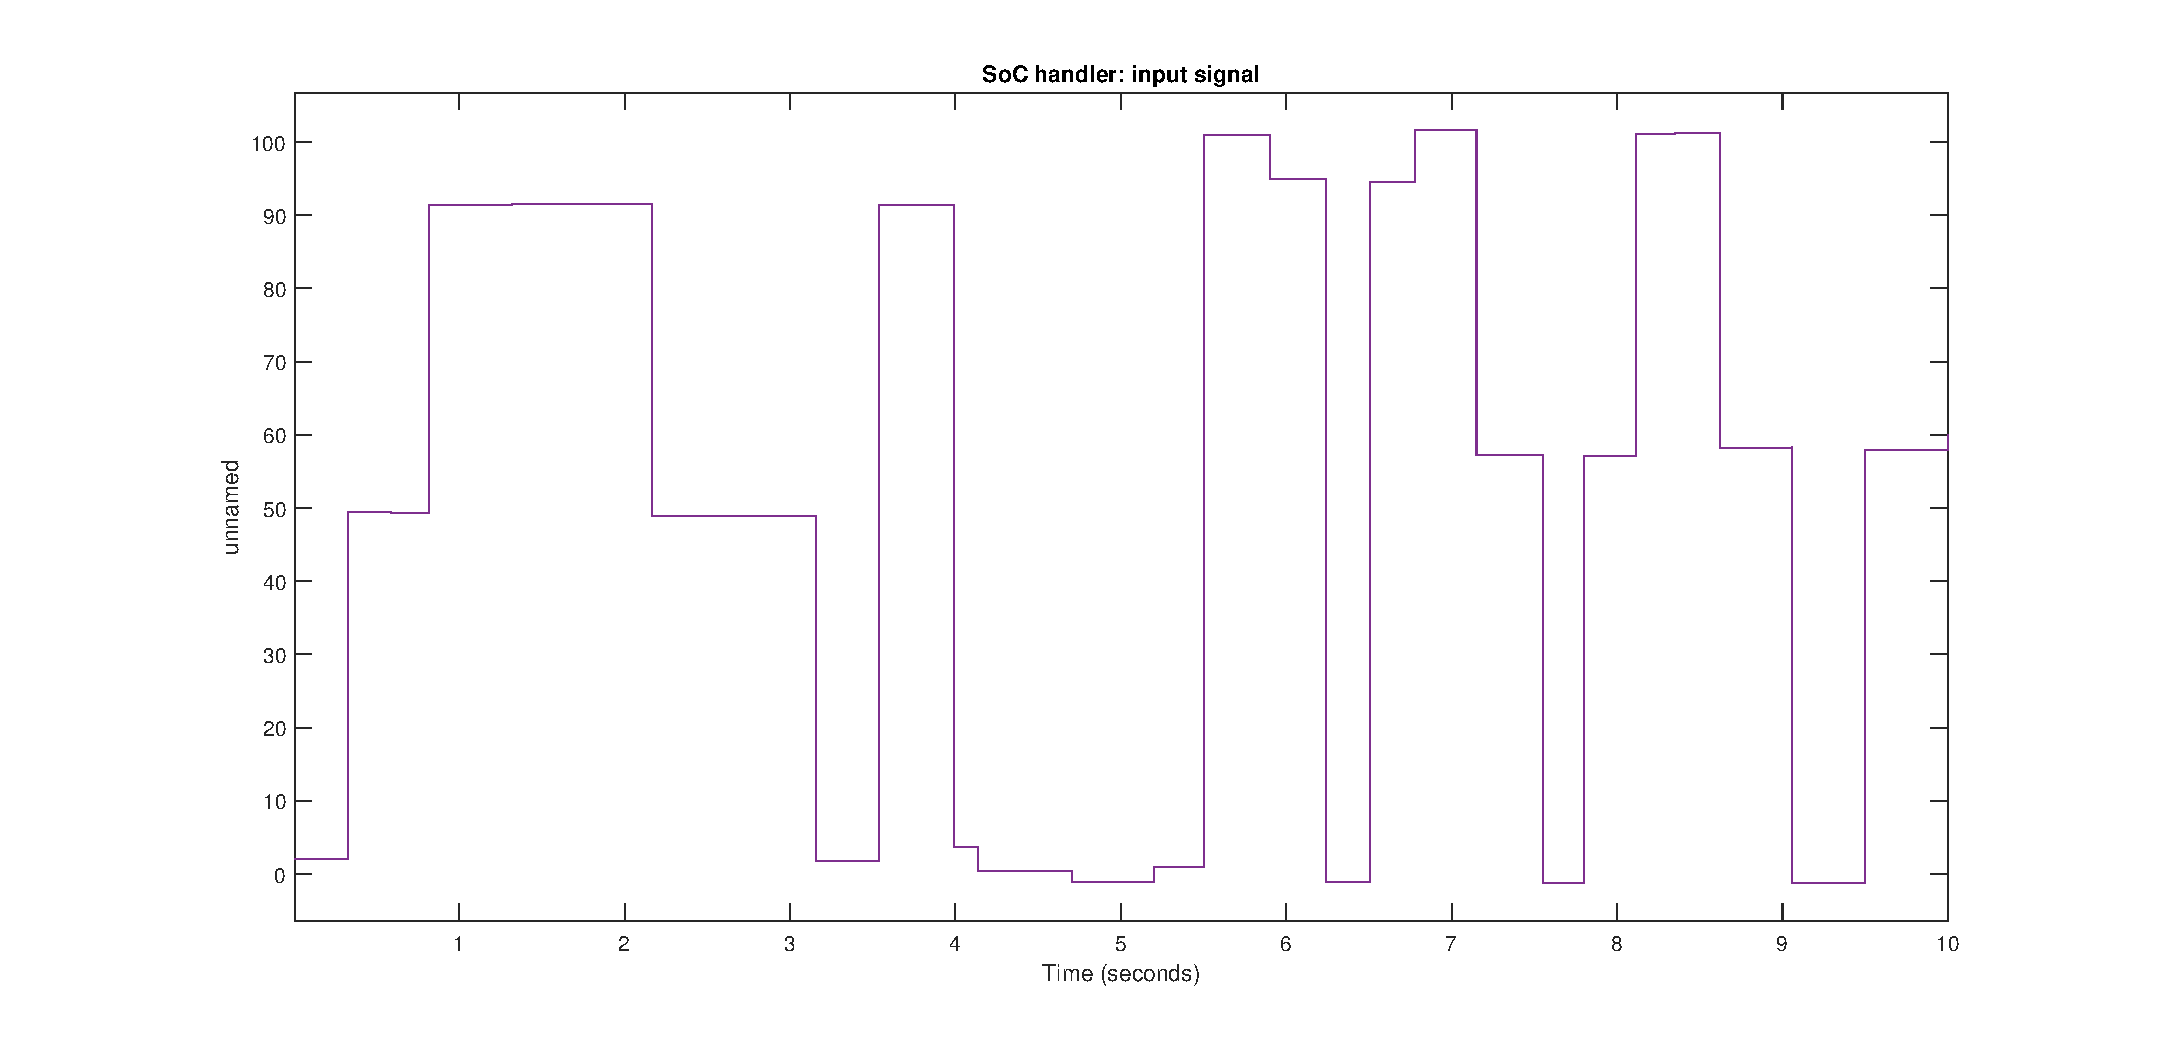
\includegraphics[scale=0.34]{SoC_handle_input.eps}
	\caption{Input fed to the SoC handler }
	\label{SoC_handle_input}
\end{figure}
\begin{figure}[!hbt]
	\centering
	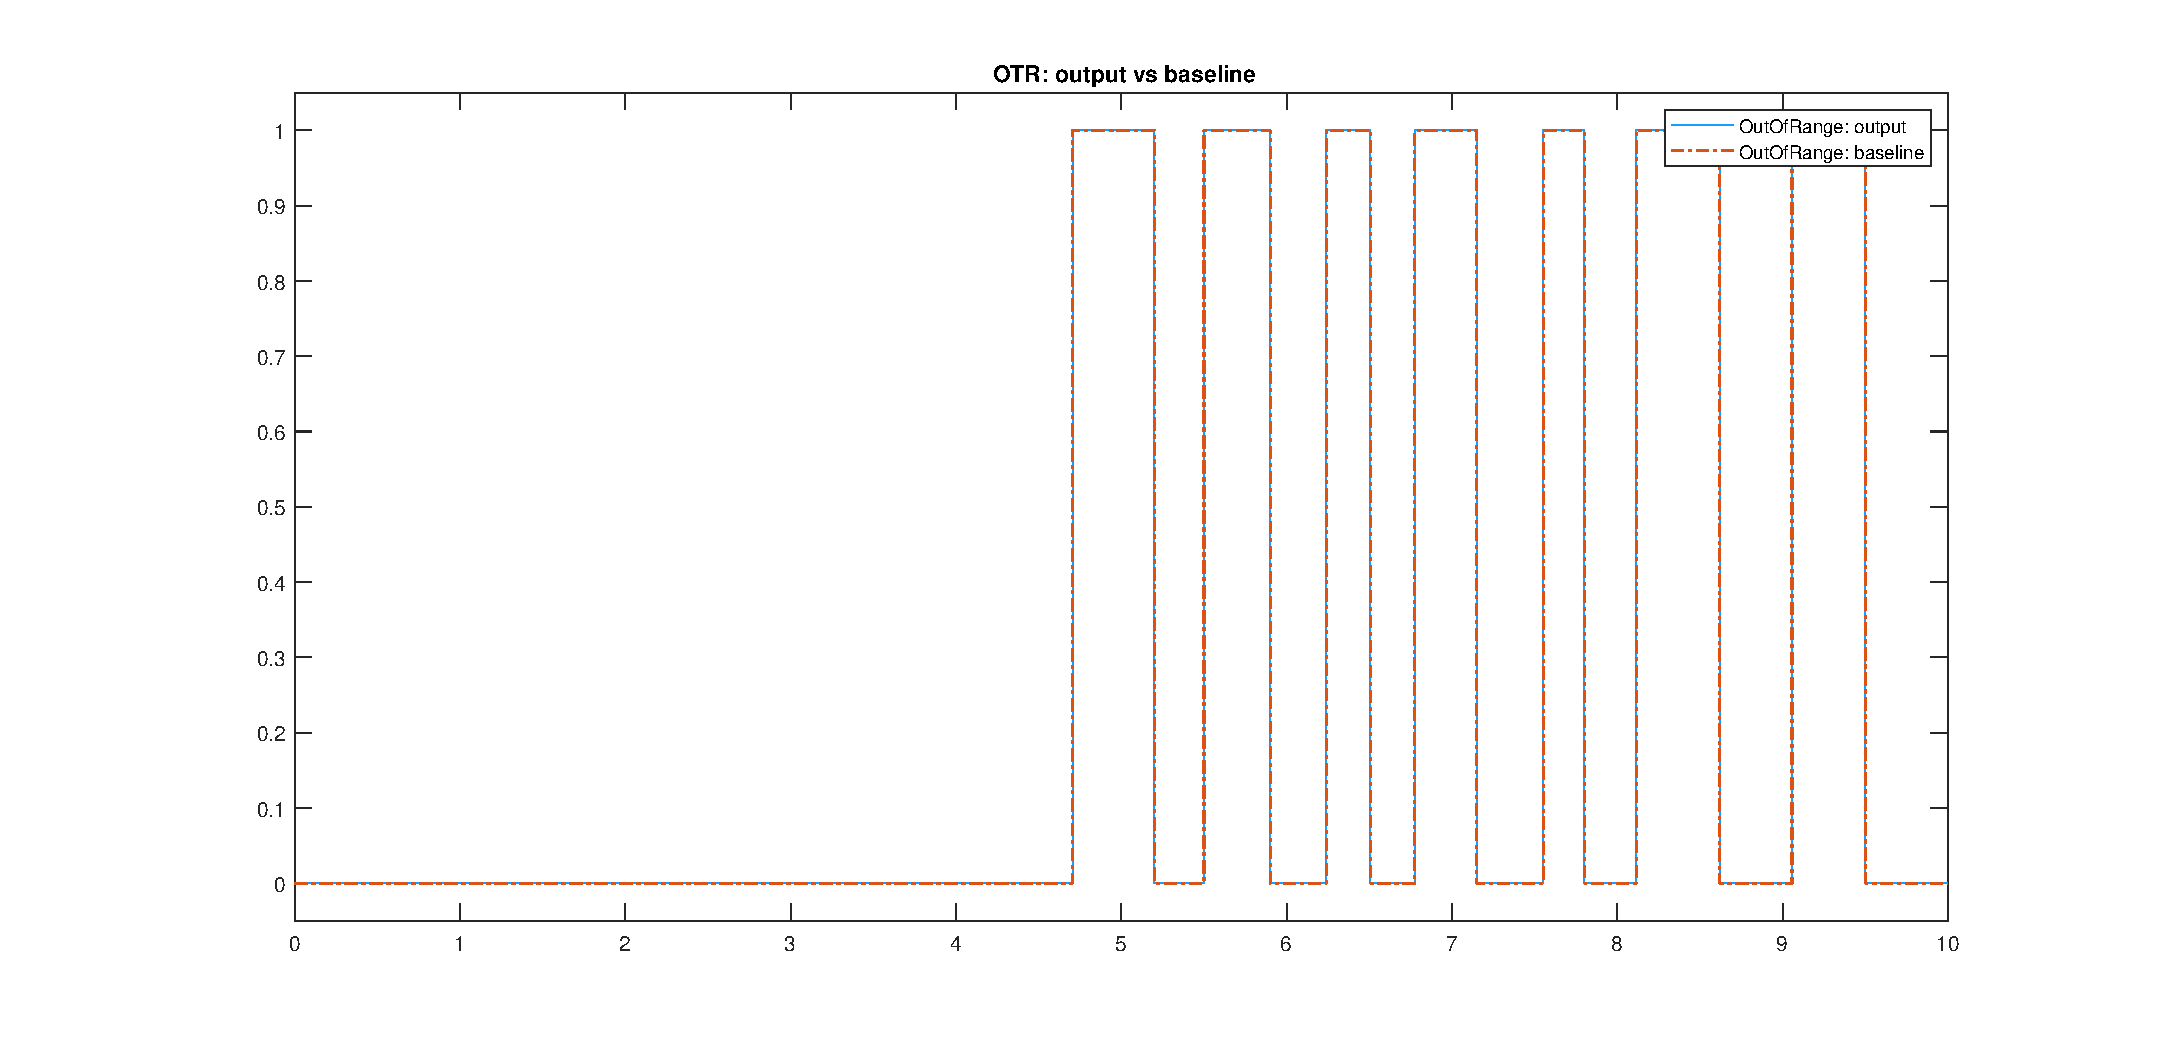
\includegraphics[scale=0.4]{OTR_baseline_result.eps}\hfill
	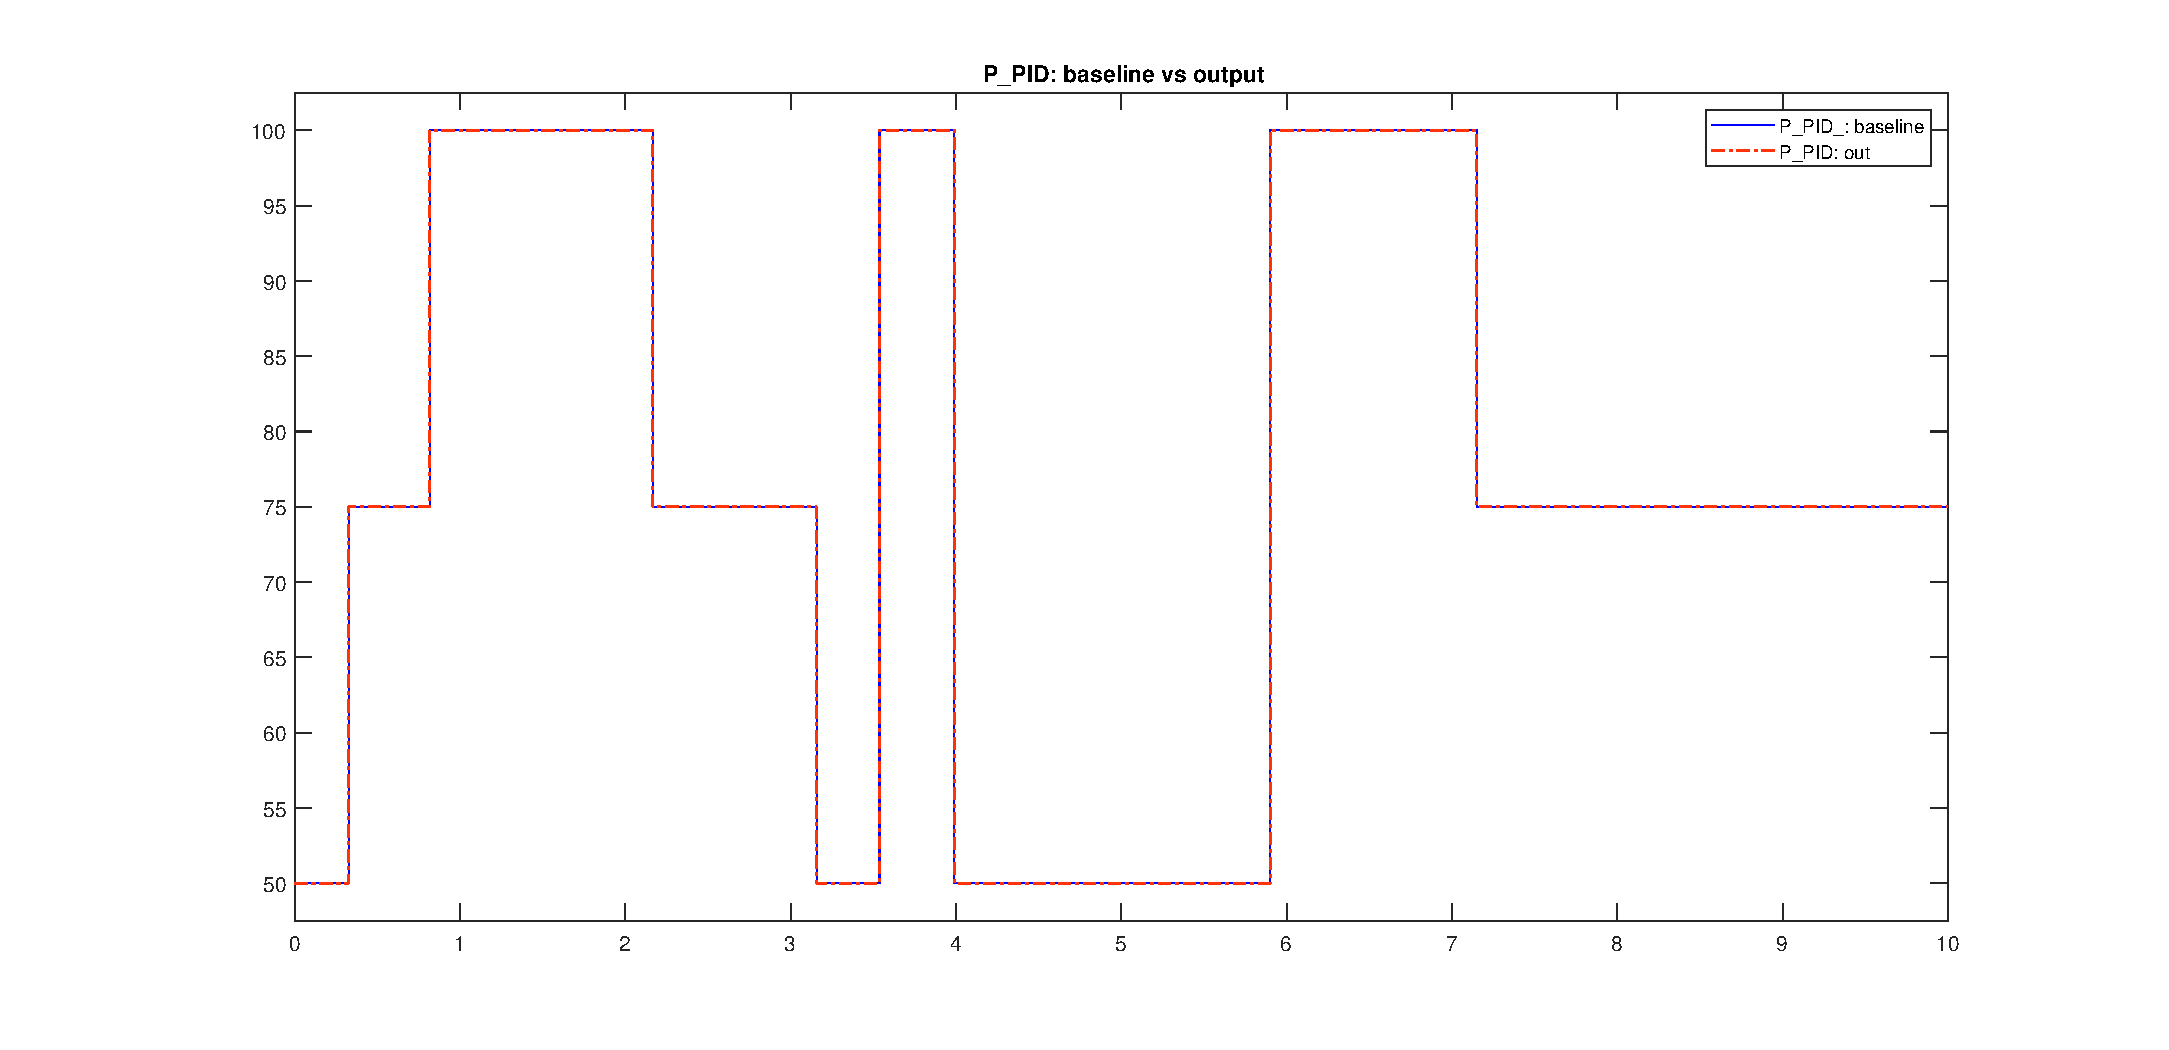
\includegraphics[scale=0.4]{PidP_baseline_result.eps}
	\caption{OTR output vs baseline (up) PID::P output vs baseline (down)}
	\label{OTR_baseline_result}
\end{figure}
We also tested the behaviour of this signal. In Fig.\ref{SoC_handle_input} you can deduce from the input signal (second half of the signal) that we wanted to test that regardless the state in wich we were and the previous value of the SoC signal, the OTR signal would raise when expected to.
In Fig.\ref{OTR_baseline_result} you can see that the output signal matches the baseline, meaning a succesful test.
\FloatBarrier
\subsection{Integration test}
All these units cooperate in the same controller module, so an integration test would be necessary. In our specific case these three units do not have in common any input or output, meaning that there is no possible integration test to be performed. All theese units are meant to condition the PID behaviour, so in order to perform an integration test the PID would have to be involved. Since we assume the PID block itself already test by MATLAB there is no point in testing the PID behaviour when not regulating a plant model.
According to the previous affirmations we decided to let the integration test coincide with the MIL test, in order to test the behaviour of the whole controller.

\section{MIL}
\section{SIL}
\section{PIL}


\chapter{Conclusion}
	
	
\end{document}